\chapter*{Lista 2}
\addcontentsline{toc}{chapter}{Lista 2}
\chaptermark{}


% Inicio da Lista de Exercícios 
\begin{enumerate}[leftmargin=*]


\item 
Sejam $B_1,\ldots, B_n$ eventos independentes. 
Mostre que 
	\[
		\P \left( \bigcup_{i=1}^n B_i \right)
		=
		1- \prod_{i=1}^n [1-\P(B_i)].
	\]


\item 
Qual é a quantidade mínima de pontos que um espaço de
probabilidade $(\Omega,\F,\P)$ deve ter para que possa
existir $n$ eventos independentes $B_1,\ldots,B_n$ 
que não tenham probabilidade zero ou um. 


\item Se $\{A_n\}$ é uma sequência de eventos independentes,
mostre que 
	\[
		\P \left( \bigcap_{i=1}^n A_n \right)
		=
		\prod_{n=1}^{\infty} \P(A_n).
	\]



\item 
Considere o espaço de probabilidade $([0,1],\mathscr{B}([0,1]),\lambda)$,
onde $\lambda$ é a medida de Lebesgue em $[0,1]$.
Seja $X:[0,1]\to\R$ a v.a. dada por $X(\omega)=\omega$.
	\begin{itemize}
		\item[a)]
		Existe alguma variável aleatória que é independente de 
		$X$ e não constante quase certamente ?
		
		\item[b)] Defina a v.a. $Y=X(1-X)$. Construa uma v.a.
		$Z$ tal que $Z$ e $Y$ sejam independentes.
	\end{itemize}



\item 
Suponha que $X$ seja uma variável aleatória.
	\begin{itemize}
		\item[a)] 
		Mostre que a v.a. $X$ é independente de si mesma 
		se, e somente se, existe uma constante $c$ tal que 
		$\P(X=c)=1$.
		
		\item[b)]
		Se existe uma função mensurável 
		$g:(\R,\mathscr{B}(\R))\to(\R,\mathscr{B}(\R))$
		tal que $X$ e $g(X)$ são independentes, então prove que
		existe uma constante $c$ tal que $\P(g(X)=c)= 1$. 				
	\end{itemize}	 
		
		
\item 
$^*$ Seja $\{X_k,k\in\N\}$ uma sequência de v.a's iid com distribuição
comum $F$. Seja $\pi$ uma permutação de $\{1,\ldots,n\}$. 
Mostre que 
	\[
		(X_1,\ldots,X_n) 
		\,{\buildrel d \over =}\, 
		(X_{\pi(1)},\ldots,X_{\pi(n)}),
	\]
onde ${\buildrel d \over =}$ significa que os dois vetores
têm a mesma distribuição conjunta. 



\item 
Se $A,B,C$ são eventos independentes, mostre que 
ambos $A\cup B$ e $A\setminus B$ são independentes de 
$C$.



\item Se $X$ e $Y$ são variáveis aleatórias independentes
e $f,g:\R\to\R$ são funções mensuráveis porque $f(X)$ e $g(Y)$
são independentes ?
\\
(Nenhuma conta é necessária).




\item
Suponha que $\{A_n\}$ é uma sequência de eventos independentes
satisfazendo $\P(A_n)<1$, para todo $n\in \N$. Mostre que 
	\[
		\P \left( \bigcup_{i=1}^n A_n \right) = 1
		\quad
		\Longleftrightarrow
		\quad
		\P(\limsup A_n) =1.
	\]
Dê um exemplo mostrando que a condição $\P(A_n)<1$ 
não pode ser removida.


\item 
Suponha que $\{X_n, n\in\N\}$ seja uma sequência de variáveis 
aleatórias independentes. Mostre que 
\[
	\P \left(  \sup_{n\in\N} X_n <\infty  \right)=1
	\quad
	\Longleftrightarrow
	\quad
	\sum_{n=1}^{\infty} \P(X_n>M) <\infty,\quad 
	\text{ para algum}\ M>0.
\]



\item
Use o Lema de Borel-Cantelli para mostrar que dada 
qualquer sequência de v.a.'s $\{X_n, n\in\N\}$, tomando valores 
reais, existe uma sequência 
$\{c_n\}$ (que não depende da sequência $\{X_n\}$) 
tal que 
	\[
		\P \left( \lim_{n\to\infty} \frac{X_n}{c_n}=0 \right)=1.
	\]
Dê uma descrição precisa das possíveis escolhas da sequência $c_n$.



\item 
O seguinte resultado é útil para ser usado juntamente 
com a Lei Zero-Um de Borel: suponha que $\{a_n\}$ 
e $\{b_n\}$ sejam duas sequências de números reais
não-negativos, satisfazendo $a_n \sim b_n$, 
isto é, $a_n/b_n\to 1$, quando $n\to\infty$.
Mostre que 
	\[	
		\sum_{n=1}^{\infty} a_n <\infty
		\quad
		\Longleftrightarrow
		\quad
		\sum_{n=1}^{\infty} b_n <\infty.
	\]	




\item 
Seja $\{X_n, n\in\N\}$ uma sequência de v.a.'s iid com
	\[
		\P(X_1=1)=p=1-\P(X_1=0).
	\]
Qual é a probabilidade que o padrão $1,0,1$ apareça
infinitas vezes ? 
\\
(Dica. Considere os eventos $A_k=\{X_k=1,X_{k+1}=0,X_{k+2}=1\}$ e 
olhe para a sequência $A_1,A_4,A_7,\ldots$).



\item 
Em uma sequência de v.a.'s de Bernoulli $\{X_n, n\in\N\}$
com 
	\[
		\P(X_n=1)=p=1-\P(X_n=0).
	\]
Seja $A_n$ o evento ocorrem $n$ uns consecutivos entre as 
observações $2^n$ e $2^{n+1}$. Mostre que se $p \geq 1/2$,
então $A_n$ ocorre infinitas vezes com probabilidade 1.
\\
Dica. Prove algo como 
\[
	\P(A_n) \geq 
	1-(1-p^n)^{\frac{2^n}{n}}
	>
	1-e^{-\frac{(2p)^n}{2n}}.		
\]


\item 
A probabilidade da convergência de uma sequência de 
v.a's independentes é igual a zero ou um. 
Se a sequência $\{X_n\}$ é iid e não constante 
com probabilidade 1, temos que 
	\[
		\P(X_n \ \text{converge}) =0.
	\]  








\item
Este exercício está relacionado ao Exemplo ???
{\bf (Comportamento de v.a.'s com distribuição exponencial)}.
	\begin{itemize}


		\item[a)]
		Suponha que $\{X_n,n\geq 1\}$ são v.a.'s iid e 
		suponha que $\{a_n\}$ é uma sequência de números 
		reais. Mostre que 
			\[
				\P(\limsup \{X_n>a_n\})
				=
				\begin{cases}
					0,&\text{se}\ \sum_{n=1}^{\infty} \P(X_1>a_n)<\infty;
					\\[0.3cm]
					1,&\text{se}\ \sum_{n=1}^{\infty} \P(X_1>a_n)=\infty;
				\end{cases}
			\]


		
		\item[b)] 
		Suponha que $\{X_n,n\in\N\}$ são v.a.'s iid com distribuição 
		normal padrão $N(0,1)$. Mostre que 
			\[
				\P\left( 
				\limsup_{n\to\infty} \frac{|X_n|}{\sqrt{\log n}}
				=\sqrt{2}  
				\right)
				=1
			\]
		Dica: Reveja ou prove que 
			\[
				\lim_{n\to\infty}
				\frac{\P(X_n>x)}{n(x)/x}=1,
			\]
		onde $n(x)$ denota a densidade de uma v.a. normal
		padrão.



		\item[c)]
		Suponha que $\{X_n, n\in\N\}$ seja uma sequência de v.a.'s 
		iid com distribuição de Poisson com parâmetro $\lambda$. 
		Prove que
			\[
				\frac{\lambda^n}{n!}e^{-\lambda}
				\leq
				\P(X_1\geq n)
				\leq
				\frac{\lambda^n}{n!}
			\]			
		e portanto 
			\[
				\P\left( 
				\limsup_{n\to\infty} \frac{X_n}{\log(\log n)}=1 
				\right)
				=1.
			\]
	\end{itemize}











\item 
Se um evento $A$ é independente de um $\pi$-sistema
$\mathcal{C}$ e $A\in \sigma(\mathcal{C})$, então 
$\P(A)$ é igual a zero ou um.









\item Dê um exemplo simples mostrando que duas 
variáveis aleatórias $X$ e $Y$ podem ser independentes
em $(\Omega,\F,\P_1)$, mas dependentes em $(\Omega,\F,\P_2)$.













\item Exemplos e Contra-exemplos.
	\begin{itemize}
		\item[a)]
		Seja $\Omega=\{1,2,3,4\}$ com cada um de seus pontos 
		tendo probabilidade $1/4$. Seja $A_1=\{1,2\}$, 
		$A_2=\{1,3\}$ e $A_3=\{1,4\}$. Mostre que quaisquer
		pares de eventos de $A_1,A_2$ e $A_3$ são independentes
		mas $A_1,A_2$ e $A_3$ não são independentes.
		
		\item[b)] 
		Seja $\{A_i, 1\leq i\leq 5\}$ uma partição mensurável de 
		$\Omega$ tal que $\P(A_1)=\P(A_2)=\P(A_3)=15/64$, 
		$P(A_4)=1/64$, $\P(A_5)=18/64$. Defina 
		$B=A_1\cup A_4$, $C=A_2\cup A_4$ e $D=A_3\cup A_4$. 
		Mostre que 
			\[
				\P(B\cap C\cap D) = \P(B)\P(C)\P(D)
			\] 
		mas que $B,C$ e $D$ não são independentes.
		
		\item[c)]
		Sejam $X_1,X_2$ variáveis aleatórias independentes
		assumindo apenas os valores $+1$ e $-1$ com probabilidade
		$1/2$. As variáveis aleatórias $X_1,X_2$ e $X_1X_2$ são 
		dois-a-dois independentes ? 
		A coleção $X_1,X_2, X_1X_2$ é independente ?
	\end{itemize}







\item Suponha que $\{A_n\}$ é uma sequência de eventos
	\begin{itemize}
		\item[a)]
		Se $\P(A_n)\to 1$, quando $n\to\infty$, mostre que 
		existe uma subsequência $\{n_k\}$ tendendo a infinito
		tal que $\P(\cap_{k} A_{n_k})>0$.
		\\
		(Dica. Use o Lema de Borel-Cantelli).
		
		
		\item[b)]
		Mostre que o seguinte é falso. Dado $\varepsilon>0$
		tal que $\P(A_n)\geq \varepsilon$ segue que existe uma subsequência
		$\{n_k\}$ tendendo a infinito tal que $\P(\cap_k A_{n_k})>0$.		
		
		
	\end{itemize}








\item 
Suponha que $\{A_n\}$ é uma sequência de eventos 
independentes tal que 
	\[
		\sum_{n=1}^{\infty}
		\left( 
			\min\{ \P(A_n), 1-\P(A_n) \}
		\right)	
		=\infty.
	\]
Mostre que $\P$ é uma medida de probabilidade 
não atômica.





\item Suponha que $\{A_n\}$ são eventos independentes.
	\begin{itemize}
		\item[a)]
		Se para cada $k\in\N$ temos 
			\[
				\sum_{n=k}^{\infty} 
				\P \left( A_n \left| \quad \bigcap_{i=k}^{n-1} A_i^c\right. \right)
				=\infty
			\]		
		Mostre que 
			\[
				\P(\limsup A_n) =1.
			\]
		
		\item[b)] Para o item anterior é suficiente assumir apenas que 
			\[
				\sum_{n=k}^{\infty} 
				\P \left( A_n \left| \quad  \bigcap_{i=1}^{n-1} A_i^c\right. \right)
				=\infty \ \ ?
			\]		
			
		\item[c)] 
		Mostre que 
			\[
				\P(\limsup A_n) =1
				\quad
				\Longleftrightarrow
				\quad
				\sum_{n=1}^{\infty} \P(A\cap A_n)
				=\infty,
			\]
		para todo evento $A$ tal que $\P(A)>0$.	
		
	\end{itemize}









\item Seja $(\Omega,\F,\P)$ um espaço de probabilidade e 
$\{A_n\}$ uma sequência arbitrária de eventos satisfazendo 
$\P(A_n)\geq \varepsilon>0$.
Mostre que $\P(\limsup A_n)\geq \varepsilon$.








\item 
Use o Teorema de Renyi para mostrar que se 
$\{X_n, n\geq 1\}$ é uma sequência iid com função distribuição
comum contínua então 
	\[
		\P\left( \limsup \left\{ X_n = \max_{1\leq i\leq n}\{X_i\}\right\} \right)
		=1.
	\]






\item 
(Barndorff-Nielson) Suponha que $\{A_n\}$ é uma sequência
de eventos tal que 
\[
	\lim_{n\to\infty} \P(A_n)=0,
	\qquad
	\sum_{n=1}^{\infty} \P(A_n\cap A_{n+1})<\infty.
\]
Prove que $\P(\limsup A_n)=0$. 
\\
(Dica. Decomponha $\cup_{j=n}^m A_j$ para $m>n$.)














\item 
Se $\{X_n, n\in\N\}$ são v.a.'s independentes, mostre que
o {\bf raio de convergência} de uma série de potências aleatória 
da forma 
	\[
		\sum_{n=1}^{\infty} X_n z^n
	\]
é constante (possivelmente infinito) com probabilidade um.
\\
Dica. O raio de convergência de uma série de potências 
$\sum_{n=1}^{\infty} c_nz^n$ é dado por 
	\[
		R^{-1} = \limsup_{n\to\infty} |c_n|^{\frac{1}{n}}.
	\]





\item 
Mostre que $\{X_n, n\in\N\}$ são independentes se 
$\sigma(X_1,\ldots,X_{n-1})$ 
é independente de $\sigma(X_n)$ para cada $n\geq 2$.









\item 
Seja $\Omega =\{1,\ldots, r\}^n$ o produto cartesiano de 
$n$ cópias de $\{1,\ldots, r\}$. 
Podemos pensar em $\Omega$ como 
	\[
		\Omega 
		=
		\{(x_1,\ldots,x_r): x_i\in\{1,\ldots r\}\ \forall i=1,\ldots,n\}
	\]
 Suponha que seja $\P$ seja
uma medida de probabilidade neste espaço tal que todo ponto 
de $\Omega$ tem a mesma probabilidade. 
Defina as seguintes variáveis aleatórias 
(projeção na $i$-ésima coordenada)
	\[
		X_i\Big((x_1,\ldots,x_n) \Big) = x_i,
		\qquad
		\forall i=1,\ldots,n.
	\]
Prove que as variáveis aleatórias $X_1,\ldots,X_n$
são independentes.




























\item Este exercício é sobre o Exemplo de Expansões Diádicas.
	\begin{itemize}
	\item[a)]
	Defina $A=\limsup \{d_{2n}=0 \}$ e $B=\limsup\{d_{2n+1}=1\}$.
	Mostre que $A$ e $B$ são independentes.
	
	\item[b)] 
	Denote por $l_n(\omega)$ o comprimento da sequência consecutiva
	de zeros, da expansão diádica de $\omega$, 
	começando do dígito $d_n(\omega)$, isto é,
		\[
			l_n(\omega)
			=
			\begin{cases}
				k,&\text{se}\ k\geq 1 \ \text{e}\ 
					d_n(\omega)=0,\ldots,d_{n+k}(\omega)=1.
				\\
				0,&\text{se} \ d_n(\omega)=1.
			\end{cases}
		\]
	Mostre que 
		\[
			\P(l_n=k) =\frac{1}{2^{k+1}},
			\qquad
			\P(l_n\geq r) = \frac{1}{2^r}.
		\]
		
	\item[c)] 
	Mostre que $\{l_n=0,n\geq 1\}$ são eventos independentes.
	
	\item[d)] 
	Mostre que $\P(\limsup \{l_n=0\})=1$.
	
	\item[e)]
	Mostre que os eventos $\{l_n=1, n\geq 1\}$ não são 
	independentes, mas os eventos $\{l_{2n}=1, n\geq 1\}$
	são. Em seguida, prove que  
		\[
			\P(\limsup \{l_{2n}=1\}) =1,
			\qquad
			\text{logo}
			\qquad
			\P(\limsup \{l_{n}=1\}) =1,		
		\]
	
	\item[f)]
	Seja $\log_2 n$ o logaritmo de $n$ na base 2. 
	Mostre que 
		\[
			\P\left(
				\limsup_{n\to\infty} \frac{l_n}{\log_2 n}\leq 1
			\right)
			=1.
		\]
	Dica. Mostre que 
		\[
			\sum_{n=1}^{\infty}
			\P(l_n>(1+\varepsilon)\log_2 n)<\infty
		\]
	e use o Lema de Borel-Cantelli. Então substitua $\varepsilon$ 
	por $\varepsilon_k\downarrow 0$.
	
	\item[g)] 
	Mostre que 
		\[
			\P\left(
				\limsup_{n\to\infty} \frac{l_n}{\log_2 n}\geq 1
			\right)
			=1.
		\]
	Dica. Seja $r_n =\log_2 n$ e defina uma sequência 
	de inteiros não negativos $n_k$ como segue:
	$n_1=1$, $n_2=1+r_1,\ldots, n_{k+1}=n_k+r_{n_k}$, com 
	$n_{k+1}-n_{k}=r_{n_k}$.
	Observe que 
		\[
			\{l_{n_k}\geq r_{n_k}\}\in 
			\mathscr{B}(d_i, n_k\leq i <n_{k+1})
		\]
	e assim os eventos $\{l_{n_k}\geq r_{n_k}\}$ para
	$k\geq 1$ são independentes. Use a Lei Zero-Um de Borel
	para mostrar que 
		\[
			\P(\limsup \{ l_{n_k} \geq r_{n_k} \}) = 1
		\]
	e consequentemente 
		\[
			\P(\limsup \{ l_{n} \geq r_{n} \}) = 1.
		\]
		
	\end{itemize}






























\item Suponha que $\{A_n, n\geq 1\}$ é uma sequência de eventos 
tais que para algum $\delta>0$ temos 
	\[
		\P(A_n)\geq \delta >0, \ \forall n\geq 1.
	\]
Mostre que $\limsup A_n \neq \emptyset$.
Use este fato para mostrar com poucos cálculos que em 
uma sequência infinita de experimentos de Bernoulli, 
existe um número infinito de sucessos com probabilidade
um.






\item 
Seja $(\Omega,\F,\P)$ um espaço de probabilidade e 
suponha que $A,B$ são dois eventos independentes.
Se $\P(B)\leq 1/2\leq \P(A)$ mostre que 
$\P(A\cup B)\geq 3/4$.






\item {\bf Truque da Raíz Quadrada}. 
Seja $(\Omega,\F,\P)$ um espaço de probabilidade. 
Suponha que $\preceq$ seja uma ordem parcial em $\Omega$.
Dizemos que $A\in\F$ é um evento crescente, 
se para todo par $\omega,\omega'$ tal que 
$\omega\preceq \omega'$, temos 
$1_{A}(\omega)\leq 1_{A}(\omega')$.

Assuma que a medida de probabilidade $\P$ é tal que
para todo par de eventos crescentes $A,B\in\F$ temos
	\begin{equation}\label{eq-exercicio-truque-raiz}
		\P(A\cap B) -\P(A)\P(B) \geq 0.
	\end{equation}
%
Sejam $A_1,\ldots,A_n$ eventos crescentes e equiprováveis tais que 
$A = \cup_{i=1}^n A_i$, então 
	\[
		\P(A_i)\geq 1-[1-\P(A)]^{\frac{1}{n}}.
	\]








\item {\bf Os Números de Ramsey}. 
O objetivo deste exercício é usar o ``Método Probabilístico''
para obter uma cota inferior dos números de Ramsey. 

{\bf Grafo.} Um grafo é um par ordenado $G=(V,E)$,
onde $V$ é um conjunto arbitrário (chamado conjunto de vértices de $G$)  
e $E$ é um conjunto formado por pares não-ordenados de $V$, 
(chamado conjunto de arestas de $G$).
Um exemplo de grafo é o grafo completo em $n$ vértices, 
chamado de $K_n$, neste grafo
$V\equiv V_n =\{1,\ldots,n\}$ e 
$E\equiv E_n =\{\{i,j\}: i,j\in \{1,\ldots,n\} \ \text{e}\ i\neq j  \}$.
Abaixo temos uma representação de $K_7$
%%%  Figura sobre Inversa Generalizada
\begin{center}
\begin{figure}[!htb]
\centering
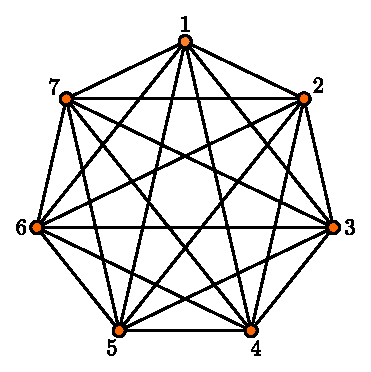
\includegraphics[width=0.4\textwidth]{Figuras/grafo-k7.pdf}
\caption{Uma representação de $K_7$.}
\label{Rotulo}
\end{figure}
\end{center}
%%%

{\bf Colorações de $K_n$.}
Uma coloração de $K_n=(V_n,E_n)$ em duas cores 
é uma função $c:E_n\to \{0,1\}$.
Seja $e\in E_n$ uma aresta de $K_n$. 
Dizemos que $e$ está colorida de azul se $c(e)=0$, 
caso $c(e)=1$ vamos dizer que $e$ está colorida de vermelho.

Fixada uma coloração $c$ de $K_n$ e um número natural $k<n$, 
dizemos que $K_n$ possui um subgrafo monocromático
{\bf azul} $K_k$, se existem $k$ vértices 
$\{v_1,\ldots,v_k\}\subset \{1,\ldots,n\}$
tais que $c(\{v_i,v_j\})=0$ para todo $i,j=1,\ldots,k$
com $i\neq k$. Analogamente definimos $K_k$ 
monocromático {\bf vermelho}.


O número de Ramsey $R(k,l)$ é o menor inteiro
$n$ tal que para qualquer coloração $c:E_n\to\{0,1\}$
de $K_n$ possui um subgrafo $K_k$ monocromático azul 
ou um subgrafo $K_l$ monocromático vermelho.

























\end{enumerate}